
\chapter{ಗ್ರೇಟ್​ ಆರ್ಕ್ ಎಂದರೇನು?}

ಲ್ಯಾಂಬಟನ್​ರವರೂ ಸಹ ಭೂಕ್ಷೇತ್ರ ಗಣಿತದಲ್ಲಿ ಅಪಾರ ಆಸಕ್ತಿ ಇದ್ದವರು. ಭೂಮಿಯ ನಿಜವಾದ ಗಾತ್ರವನ್ನು ಪ್ರಾಯೋಗಿಕವಾಗಿ ಕಂಡುಹಿಡಿಯುವ ಕಾರ್ಯವನ್ನು ತಾನೂ ಮಾಡಬೇಕು ಎಂದು ಚಿಂತಿಸಿದರು. ಈ ಪ್ರಯೋಗ ಕಾರ್ಯಕ್ಕೆ ಅವರಿಗೆ ಅತ್ಯಂತ ಉದ್ದವಾದ ರೇಖಾಂಶ ನೇರದಲ್ಲಿನ ವೃತ್ತ ಕಂಸ ಭೂಭಾಗವು ಬೇಕಾಗಿತ್ತು. ಆ ಭೂಭಾಗವು ಸಮಭಾಜಕಕ್ಕೆ ಸಮೀಪದಲ್ಲಿ ಇರುವುದು ಅಪೇಕ್ಷಣೀಯವಾಗಿತ್ತು. ಬ್ರೀಟೀಷರ ಸ್ವಾಧೀನದಲ್ಲಿ ಅಂತಹ ಸೂಕ್ತವಾದ ಸ್ಥಳದ ಲಭ್ಯತೆಯು ಭಾರತ ಬಿಟ್ಟರೆ ಬೇರೆಲ್ಲೂ ಇರಲಿಲ್ಲ. ಆದ್ದರಿಂದ ಲ್ಯಾಂಬ್​ಟನ್​ರವರು ಆರ್ಕ್\break ಮೆಸರ್​ಮೆಂಟ್​ ಕಾರ್ಯವನ್ನು ಭಾರತದಲ್ಲಿಯೂ ಮಾಡಬೇಕೆಂದು ನಿರ್ಧರಿಸಿದರು. ಈ ಉದ್ದೇಶವನ್ನು ದೃಷ್ಟಿಯಲ್ಲಿಟ್ಟುಕೊಂಡೇ, ಲ್ಯಾಂಬ್​ಟನ್​ರವರು ತಮ್ಮ ‘ಮೆರಿಡಿಯನಲ್​ ಆರ್ಕ್ ಮೆಜರ್​ಮೆಂಟ್​ ಮತ್ತು ಟ್ರಿಗನಮಿಟ್ರಿಕಲ್​ ಸರ್ವೇ’ಗಾಗಿ ವರದಿಯನ್ನು ಸಲ್ಲಿಸಿದ್ದರು.\break ಕನ್ಯಾಕುಮಾರಿಯಿಂದ ಹಿಮಾಲಯದವರೆಗೆ, ಅಂದಾಜಿನ $78^\circ$ ರೇಖಾಂಶ ರೇಖೆ ನೇರದಲ್ಲಿ, ದಕ್ಷಿಣೋತ್ತರವಾಗಿ ಸಾಗುವ ಸರಣೀ ತ್ರಿಭುಜಗಳ ಪಟ್ಟಿಯನ್ನು ರಚಿಸಲು ತೀರ್ಮಾನಿಸಿದರು. ಈ ಸರಣೀ ತ್ರಿಭುಜಗಳ ಪಟ್ಟಿಯ ರೇಖಾಂಶ ನೇರವನ್ನು ‘ಗ್ರೇಟ್​ ಆರ್ಕ್’ ಎಂದು ಕರೆಯಲಾಗಿದೆ.

`ಗ್ರೇಟ್​ ಆರ್ಕ್’ ಅಂದರೆ ಏನು ಎಂದು ತಿಳಿದುಕೊಳ್ಳುವ ಮೊದಲು, ‘ಗ್ರೇಟ್​ ಸರ್ಕಲ್​’ ಎಂದರೇನು ಅಂತ ಮೊದಲು ತಿಳಿದುಕೊಳ್ಳಬೇಕು. ‘ಗ್ರೇಟ್​ ಸರ್ಕಲ್​’ ಎಂದರೆ ಭೂಗೋಳದ ಹೊರಮೈ ಮೇಲೆ ಹಾಯುವ ಪೂರ್ಣ ವೃತ್ತ ಅದು. ಭೂಗೋಳಕ್ಕೆ ಒಂದು ಬಳೆ ತೊಡಿಸಿದರೆ ಕಾಣುತ್ತಲ್ಲಾ, ಆ ಬಳೆ ಅಥವ ವೃತ್ತವೇ ಮಹಾ ವೃತ್ತ ಅಥವಾ ‘ಗ್ರೇಟ್​ ಸರ್ಕಲ್​’. ಈ ಮಹಾ ವೃತ್ತದ ಕೇಂದ್ರವು ಮತ್ತು ಭೂಗೋಳದ ಕೇಂದ್ರವು ಒಂದೇ ಆಗಿರುತ್ತದೆ. ಗ್ರೇಟ್​ ಸರ್ಕಲ್​ನ ತ್ರಿಜ್ಯವೂ ಸಹ ಭೂಗೋಳದ ತ್ರಿಜ್ಯವೇ ಆಗಿರುತ್ತದೆ. ಗ್ರೇಟ್​ ಸರ್ಕಲ್​ನ ಸುತ್ತಳತೆಯೂ ಸಹ ಭೂಮಿಯ ಸುತ್ತಳತೆಯೇ ಆಗಿರುತ್ತದೆ. ಈ ಗ್ರೇಟ್​ ಸರ್ಕಲ್​ನಲ್ಲಿ ಸ್ವಲ್ಪ ಭಾಗವನ್ನಷ್ಟೇ ಭಾವಿಸಿಕೊಂಡರೆ, ಆ ಸ್ವಲ್ಪ ಭಾಗವು ‘ಗ್ರೇಟ್​ ಆರ್ಕ್’ ಆಗಿರುತ್ತದೆ. ಟ್ರೈಯಾಂಗ್ಯುಲೇಶನ್​ ಸರ್ವೇ ವಿಧಾನದ ಮೂಲಕ, ಸರಣೀ ತ್ರಿಭುಜಗಳ ಪಟ್ಟಿಯನ್ನು ಭೂಗೋಲದ ಮೇಲೆ ರಚಿಸಿದರೆ, ಆ ತ್ರಿಭುಜಗಳ ಪಟ್ಟಿಯ ಮೇಲೆ ಗ್ರೇಟ್​ ಆರ್ಕ್ ಸಿಗುತ್ತದೆ. ಹೀಗೆ, ಟ್ರಿಗನಮಿಟ್ರಿಕಲ್​ ಸರ್ವೇಯಲ್ಲಿ, ಗ್ರೇಟ್​ ಆರ್ಕ್‌ನ್ನು ರಚಿಸಿ, ಅಳೆದರೆ, ಗ್ರೇಟ್​ ಆರ್ಕ್‌ನ ತ್ರಿಜ್ಯವನ್ನು ಕಂಡುಹಿಡಿಯಬಹುದು. ಅದು ಭೂಮಿಯ ತ್ರಿಜ್ಯವೂ ಆಗಿರುತ್ತದೆ. ಮೂಲ ಉದ್ದೇಶ ಭೂಮಿಯ ವಕ್ರತೆಯ ಸ್ಪಷ್ಟ ಆಕಾರವನ್ನು ನಿರ್ಧರಿಸುವುದು. ಆಗ ಭೂಗಾತ್ರವು ಲಭಿಸುತ್ತದೆ. ಇದು ಟ್ರಿಗನಮಿಟ್ರಿಕಲ್​ ಸರ್ವೇಯಲ್ಲಿನ ವಿಜ್ಞಾನದ ಅಂಶ. ಭೂಮಿಯ ಗಾತ್ರ, ಆಕಾರ ಅರಿಯಲು ಸರ್ವೇಯ ಪಾತ್ರ ಅಪಾರ, ಅದರಲ್ಲೂ ಟ್ರಿಗನಮಿಟ್ರಿಕಲ್​ ಸರ್ವೇಯದು ಮುಖ್ಯ ಪಾತ್ರ.

ಆದರೆ ಲ್ಯಾಂಬ್​ಟನ್​ರವರು, ತಮ್ಮ ಟ್ರಿಗನಮಿಟ್ರಿಕಲ್​ ಸರ್ವೇಯಲ್ಲಿ, ವಿಜ್ಞಾನದ ಅಂಶಕಷ್ಟೇ ಒತ್ತು ಕೊಡುವುದಿಲ್ಲ. ಪ್ರಮುಖ ಭೌಗೋಳಿಕ ಸ್ಥಾನಗಳನ್ನು ಅಂದರೆ, ಟ್ರಿಗನಮಿಟ್ರಿಕಲ್​ ಸ್ಟೇಷನ್​ಗಳನ್ನು ನಿರ್ಧರಿಸುವುದರಿಂದ, ಮ್ಯಾಪಿಂಗ್​ ಕಾರ್ಯಕ್ಕೆ ಅದರಿಂದಾಗುವ ಅನುಕೂಲ ಮತ್ತು ಅದರ ವೈಜ್ಞಾನಿಕ ಉಪಯುಕ್ತತೆ ಇವೆರಡನ್ನೂ ಸ್ಪಷ್ಟವಾಗಿ ಮನಗಂಡಿದ್ದರು. ಮ್ಯಾಪಿಂಗ್​ ಕಾರ್ಯಕ್ಕೆ ಈ ಟ್ರಿಗನಮಿಟ್ರಿಕಲ್​ ಸ್ಟೇಷನ್​ಗಳು, ನಿಯಂತ್ರಣ ಬಿಂದುಗಳಾಗಿ ಹೇಗೆ ಸಹಾಯಕವೆಂದು ತಮ್ಮ ಜತೆಗಿನ ವಿಜ್ಞಾನಿಗಳಿಗೆ ಸಮರ್ಥವಾಗಿ ಅವರು ಮನದಟ್ಟು ಮಾಡಿದರು. ಅಲ್ಲಿ ಇಲ್ಲಿ ಮಾಡುವ ಬಿಡಿ ಬಿಡಿ ಮ್ಯಾಪಿಂಗ್​ ಕಾರ್ಯದ ಬದಲಿಗೆ ಇಡೀ ಭಾರತದ ಸರ್ವೇಗೆ ಒಂದೇ ಚೌಕಟ್ಟು ಸೂಕ್ತ ಎಂದರು. ಭೂಮಿಯ ಮೇಲಿನ ಗೋಚರ ವಿವರಗಳನ್ನು ಚಿತ್ರಿಸುವ ಮ್ಯಾಪಿಂಗ್​ ಕಾರ್ಯಕ್ಕೆ ಡೀಟೈಲ್​ ಸರ್ವೇ ಎನ್ನುತ್ತಾರೆ. ಬೆಟ್ಟ ಗುಡ್ಡ, ಕೆರೆ ಕಟ್ಟೆ, ಹೊಳೆ ಹಳ್ಳ, ರಸ್ತೆ ರೈಲ್ವೆ, ಊರು ಕೇರಿ, ಪಟ್ಟಣ ನಗರ, ಗಡಿ ರೇಖೆ, ಮೇರೆ ಗುರುತು, ಹೀಗೆ ಕಣ್ಣಿಗೆ ಎದ್ದು ಕಾಣುವ ಪ್ರಮುಖಾಂಶಗಳೆಲ್ಲವನ್ನು ‘ವಿವರಗಳು’ ಅಥವಾ ‘ಡೀಟೈಲ್ಸ್’ ಎಂದು ಮ್ಯಾಪಿಂಗ್​ ಸಂದರ್ಭದಲ್ಲಿ ಕರೆಯುತ್ತಾರೆ. ಈ ಭೌಗೋಳಿಕ ವಿವರಗಳನ್ನು ಚಿತ್ರಿಸಲು ಮಾಡುವ ಸರ್ವೇಗೆ ‘ಡೀಟೈಲ್​ ಸರ್ವೇ’ ಎಂದು ಕರೆಯುತ್ತಾರೆ. ಟ್ರಿಗನಮಿಟ್ರಿಕಲ್​ ಸರ್ವೇಯ ಫ್ರೇಮ್ ವರ್ಕ್ ಇಲ್ಲದೇ ಡೀಟೈಲ್​ ಸರ್ವೇ ಮಾಡಿದರೆ, ಅಂತಹ ಡೀಟೈಲ್​ ಸರ್ವೇಯು ವಿಶ್ವಾಸಾರ್ಹ ಆಗುವುದಿಲ್ಲ ಎಂದು ಲ್ಯಾಂಬಟನ್​ರವರು ತೋರಿಸಿಕೊಡುತ್ತಾರೆ. ಎಲ್ಲಾ ಸರ್ವೇಗೂ ಗಟ್ಟಿ ಆಧಾರವನ್ನು ಒದಗಿಸುವ ಟ್ರಿಗನಮಿಟ್ರಿಕಲ್​ ಸರ್ವೇ ಕಾರ್ಯಾಚರಣೆಗೆ ಅಪಾರ ಖರ್ಚು ತಗಲುತ್ತದೆ. ಆದರೆ ಅವೈಜ್ಞಾನಿಕವಾದ ಗಣಿತ ಆಧಾರವಿಲ್ಲದ, ಬಿಡಿ ಬಿಡಿ ಸರ್ವೇ ಕಾರ್ಯಗಳ ದೋಷಯುತ ಫಲಿತಾಂಶವೂ ನಿರರ್ಥಕ. ಅಂತಹ ದೋಷಯುತವಾದ ಸರ್ವೇಗಾಗಿ ವಿನಿಯೋಗಿಸುವ ಹಣವೂ ವ್ಯರ್ಥ. ಸರ್ವೇ ಕಾರ್ಯಾಚರಣೆಯಿಂದ ಒದಗುವ ಮ್ಯಾಪು ಅದು ನಿಜಕ್ಕೆ ಹಿಡಿದ ಕನ್ನಡಿಯಾಗಿರಬೇಕು. ದೃಶ್ಯವು ಸ್ವಲ್ಪವೂ ವಿರೂಪಗೊಳ್ಳದೆ ಅದು ಭೂಮಿಯ ನೈಜ ನಿರೂಪಣೆ ಆಗಿರಬೇಕು. ಆಗ ಮಾತ್ರ ಆ ಸರ್ವೇಗೆ ಮಾನ್ಯತೆ. ಇದು ಲ್ಯಾಂಬ್​ಟನ್​ರವರ ಈ ಸರ್ವೇಯ ಪರಿಕಲ್ಪನೆ ಆಗಿತ್ತು. ಸರ್ವೇಯಲ್ಲಿನ ಉನ್ನತ ಶಿಷ್ಠತೆಗಾಗಿ ಲ್ಯಾಂಬ್​ಟನ್​ರವರ ಈ ಮಹಾ ಸರ್ವೇ ಕಾರ್ಯವನ್ನು \enginline{1818}ರಲ್ಲಿ ಅನೇಕ ವರ್ಷಗಳ ನಂತರ ಅಂತರಾಷ್ಟ್ರೀಯ ವಿಜ್ಞಾನ ಸಂಸ್ಥೆಗಳು ಗುರುತಿಸಿ, ಇದನ್ನು ಅಧಿಕೃತವಾಗಿ ‘ಗ್ರೇಟ್​ ಟ್ರಿಗನಮಿಟ್ರಿಕಲ್​ ಸರ್ವೇ ಆಫ್​ ಇಂಡಿಯ’ ಎಂದು ಕರೆದವು. ನಂತರ ಕಾಲಘಟ್ಟದಲ್ಲಿ ಜಾಗತಿಕ ಮಟ್ಟದಲ್ಲಿಯೇ ಮಹಾ ಸರ್ವೇ ಎಂದು ಗುರುತಿಸುವಂತಹ ಹೆಗ್ಗಳಿಕೆಯ ಮಾತನ್ನು ಪಡೆದ ಮ್ಯಾಪಿಂಗ್​ ಮಹಾ ಕಾರ್ಯ ಇದಾಯಿತು.

ಗ್ರೇಟ್​ ಟ್ರಿಗನಮಿಟ್ರಿಕಲ್​ ಸರ್ವೇಯನ್ನು ಟ್ರೈಯಾಂಗ್ಯುಲೇಷನ್​ ವಿಧಾನದಲ್ಲಿ, ಅಂದರೆ ತ್ರಿಭುಜೀಕರಣ ವಿಧಾನದಲ್ಲಿ ಮಾಡಲಾಗಿದೆ. ‘ತ್ರಿಭುಜೀಕರಣ’ ವಿಧಾನವೆಂದರೆ, ಭೂಮಿಯ ಮೇಲೆ ತ್ರಿಭುಜಗಳ ರಚನೆ ಮತ್ತು ಅದರಲ್ಲಿನ ಕೋನಗಳ ಅಳತೆ. ಸೈದ್ಧಾಂತಿಕವಾಗಿ ತ್ರಿಭುಜೀಕರಣ ಸರಳವಾದದ್ದು. ಕಾಗದದ ಮೇಲೆ ತ್ರಿಭುಜಾಕಾರ ಮೂಡುವಂತೆ ಮೂರು ಬಿಂದುಗಳನ್ನಿಟ್ಟು, ಆ ಮೂರು ಬಿಂದುಗಳನ್ನು ರೇಖೆಗಳಿಂದ ಸೇರಿಸಿದರೆ, ತ್ರಿಭುಜ ರಚನೆಯಗುತ್ತದೆ. ಕೋನಮಾಪಕದ ಸಹಾಯದಿಂದ ಕೋನಗಳನ್ನು ಅಳೆದು, ಅವುಗಳನ್ನು ಕೂಡಿದರೆ, ಅವುಗಳ ಮೊತ್ತವು $180^\circ$ ಇರುತ್ತದೆ. ತ್ರಿಭುಜದ ಒಂದು ಬಾಹು ಮತ್ತು ಅದರ ಮೂರು ಕೋನಗಳು ತಿಳಿದಿದ್ದರೆ, ಉಳಿದ ಎರಡು ಬಾಹುಗಳನ್ನು ಅಳೆಯದೇ ಅವುಗಳ ಅಳತೆಯನ್ನು ಗಣಿತ ಸೂತ್ರದಿಂದ ಸುಲಭವಾಗಿ ಲೆಕ್ಕಾಚಾರ ಮಾಡಬಹುದು. ಇದು ಸೈದ್ಧಾಂತಿಕವಾಗಿ ಕಾಗದದ ಮೇಲಿನ ಸುಲಭ ಕಾರ್ಯ.

ಅದೇ ರೀತಿಯಲ್ಲಿ, ಭೂಮಿಯ ಮೇಲೆ, ಪರಸ್ಪರ ಗೋಚರಿಸುವ, ತ್ರಿಭುಜ ಆಕಾರದಲ್ಲಿ ಬರುವಂತೆ, ಮೂರು ಬಿಂದುಗಳನ್ನು ಗುರುತಿಸಿದರೆ, ಭೂಮಿಯ ಮೇಲೂ ಕಾಲ್ಪನಿಕ ತ್ರಿಭುಜ ಸಿದ್ಧವಾಗುತ್ತದೆ. ಪ್ರಾರಂಭದಲ್ಲಿ ಆ ಕಾಲ್ಪನಿಕ ತ್ರಿಭುಜದ ಯಾವುದಾದರೂ ಎರಡು ಅನುಕೂಲ ಬಿಂದುಗಳ ನಡುವಿನ, ಒಂದು ಬಾಹುವನ್ನು ಆಯ್ಕೆ ಮಾಡಿಕೊಳ್ಳಬೇಕು. ಆ ಒಂದು ಬಾಹುವಿನ ದೂರವನ್ನು, ಸಾದ್ಯವಾದ ಗರಿಷ್ಟ ನಿಖರತೆಯಿಂದ ಅಳೆಯಲಾಗುತ್ತದೆ. ಹೀಗೆ ಗರಿಷ್ಠ ನಿಖರತೆಯಲ್ಲಿ ಅಳತೆ ಮಾಡಿದ ತ್ರಿಭುಜದ ಬಾಹುವನ್ನು, ‘ಬೇಸ್‌ಲೈನ್​’ ಎನ್ನುತ್ತಾರೆ. ಮತ್ತು ಆ ಬೇಸ್‌ಲೈನ್​ನ ಎರಡೂ ಬಿಂದುಗಳಿಂದ ಮೂರನೇ ಬಿಂದುವಿಗೆ, ಥಿಯಡೋಲೈಟ್​ ಎಂಬ ಕೋನ ಅಳೆಯುವ ಸರ್ವೇ ಉಪಕರಣವನ್ನು ಬಳಸಿ, ಕೋನಗಳನ್ನು ನಿಖರವಾಗಿ ಅಳೆಯಲಾಗುತ್ತದೆ. ಮೂರನೇ ಬಿಂದುವಿನಲ್ಲೂ ನಿಂತು, ಬೇಸ್‌ಲೈನ್​ನ ಎರಡು ಬಿಂದುಗಳ ನಡುವಿನ ಮೂರನೇ ಕೋನವನ್ನು ಅಳೆಯಲಾಗುತ್ತದೆ.

\begin{figure}[!htbp]
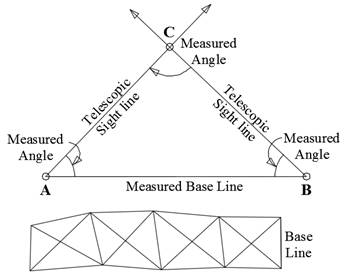
\includegraphics[scale=.7]{"images/image003.jpg"}
\caption{ತ್ರಿಭುಜೀಕರಣ}\label{chap3-fig01}
\end{figure}

ತ್ರಿಭುಜದಲ್ಲಿ \enginline{3} ಕೋನಗಳು ಮತ್ತು ಒಂದು ಬಾಹುವಿನ ಅಳತೆ ಗೊತ್ತಿದ್ದರೆ, ಆಗ ಟ್ರಿಗನಮಿಟ್ರಿಯ ‘ಸೈನ್​ ರೂಲ್​’ ಬಳಸಿ ತ್ರಿಭುಜದ ಉಳಿದ \enginline{2} ಬಾಹುಗಳ ದೂರವನ್ನು ಲೆಕ್ಕಾಚಾರದಿಂದ ಕಂಡು ಹಿಡಿಯಬಹುದು. ಹೀಗೆ ಈ ಲೆಕ್ಕಾಚಾರದಿಂದ ಕಂಡು ಹಿಡಿದ ತ್ರಿಭುಜದ \enginline{2}ನೇ ಬಾಹು ಮತ್ತು \enginline{3}ನೇ ಬಾಹುಗಳು, ಅದರ ಪಕ್ಕದ ಮುಂದಿನ ತ್ರಿಭುಜವನ್ನು ಬಿಡಿಸಲು ಬೇಸ್‌ಲೈನ್​ ಆಗುತ್ತವೆ. ಹೀಗೆ ಒಂದಾದ ಮೇಲೆ ಮತ್ತೊಂದು ತ್ರಿಭುಜಗಳನ್ನು ರಚಿಸಿದಾಗ, ತ್ರಿಭುಜದ ಸರಣೀ ಪಟ್ಟಿ ಏರ್ಪಡುತ್ತದೆ. ತ್ರಿಭುಜೀಕರಣದಲ್ಲಿ ಒಮ್ಮೆ ಮಾತ್ರ ಲೀನೀಯರ್​ ಅಳತೆಯನ್ನು ಮಾಡುವುದು. ಅದು ಆರಂಭದ ಬೇಸ್‌ಲೈನ್​ ಮೇಲೆ ಮಾತ್ರ. ನಂತರ ಉಳಿದೆಲ್ಲಾ ಅಳತೆಗಳು ಕೋನೀಯ ಅಳತೆಗಳು. ತ್ರಿಭುಜೀಕರಣದ ವಿಶೇಷತೆಯೇ ಇದು. ದಕ್ಷಿಣದ ಕನ್ಯಾಕುಮಾರಿ ಯಿಂದ ಉತ್ತರದ ಹಿಮಾಲಯದವರೆಗೂ ತ್ರಿಭುಜದ ಸರಣೀ ಪಟ್ಟಿಯನ್ನು ರಚಿಸಬಹುದು. ಈ ತ್ರಿಭುಜದ ಸರಣೀ ಪಟ್ಟಿಯ, ರೇಖಾಂಶ ನೇರವೇ ‘ಗ್ರೇಟ್​ ಆರ್ಕ್’ ಆಗುತ್ತದೆ. ಹಾಗು ಈ ತ್ರಿಭುಜದ ಶೃಂಗ ಬಿಂದುಗಳು ‘ಗ್ರೇಟ್​ ಟ್ರಿಗನಮಿಟ್ರಿಕಲ್​ ಸ್ಟೇಷನ್​’ ಗಳಾಗುತ್ತವೆ. ಸಂಕ್ಷಿಪ್ತವಾಗಿ ಹೇಳುವುದಾದರೆ ‘ಜಿಟಿಎಸ್​’ಗಳಾಗುತ್ತವೆ. ಈ ಜಿಟಿಎಸ್​ಗಳು ಮುಂದಿನ ಹಂತದ ಟೋಪೋಗ್ರಫಿಕಲ್​, ಮಿಲಿಟರಿ ಮತ್ತು ಕೆಡಸ್ಟ್ರಲ್​ ಸರ್ವೇ ಕಾರ್ಯಗಳಿಗೆ ನಿಯಂತ್ರಣ ಬಿಂದುಗಳಾಗುತ್ತವೆ. ಈ ಸರ್ವೇಯು, ತ್ರಿಭುಜಗಳ ರಚನೆಯ ಕಾರ್ಯವಾಗಿರುವುದರಿಂದ, ಇದು ಟ್ರೈಯಾಂಗ್ಯುಲೇಷನ್​ ಸರ್ವೇ ಆಗುತ್ತದೆ. ಹಾಗೆಯೇ ಈ ಸರ್ವೇಯಲ್ಲಿ, ಬಹು ಮುಖ್ಯವಾಗಿ ಟ್ರಿಗನಮಿಟ್ರಿಯ ತತ್ವವನ್ನು ಪ್ರತೀ ಹಂತದಲ್ಲೂ ಬಳಸುವುದರಿಂದ, ಇದು ಟ್ರಿಗನಮಿಟ್ರಿಕಲ್​ ಸರ್ವೇಯೂ ಹೌದು.

ಈ ಸರಣಿ ತ್ರಿಭುಜಗಳ ಪಟ್ಟಿಯು ಕೊನೆಗೊಂಡಾಗ, ಕೊನೆಯ ಬಾಹುವನ್ನು ನೇರವಾಗಿ ನೆಲದ ಮೇಲೆ, ಸರಪಳಿಯಿಂದ ಅಳೆದರೆ, ಟ್ರೈಯಾಂಗ್ಯುಲೇಷನ್​ ಕಾರ್ಯದ ನಿಖರತೆಯು ಸಿಗುತ್ತದೆ. ಹೀಗೆ, ನೆಲದ ಮೇಲೆ ನೇರವಾಗಿ ಅಳೆದ ತ್ರಿಭುಜದ ಕೊನೆಯ ಬಾಹುವನ್ನೂ ಸಹ ‘ಬೇಸ್‌ಲೈನ್​’ ಎಂದೇ ಕರೆಯುತ್ತಾರೆ. ಆದರೆ ಇದು ಪರಿಶೀಲನಾ ಬೇಸ್‌ಲೈನ್​ ಆಗಿರುತ್ತದೆ. ಪರಿಶೀಲನಾ ಬೇಸ್‌ಲೈನ್​ ಅಳತೆಯ ಜೊತೆಗೆ, ಇನ್ನೂ ಒಂದು ರೀತಿಯ ಚೆಕಿಂಗ್​ ಕಾರ್ಯ ಉಂಟು. ಆಯ್ದ ಟ್ರೈಯಾಂಗ್ಯುಲೇಷನ್​ ಬಿಂದುಗಳಲ್ಲಿ, ಖಗೋಳ ವೀಕ್ಷಣೆಯಿಂದ ಆ ಬಿಂದುಗಳ ಅಕ್ಷಾಂಶ, ರೇಖಾಂಶಗಳನ್ನು ಲೆಕ್ಕಾಚಾರ ಮಾಡಲಾಗುತ್ತದೆ. ಇದರಿಂದ ಬರುವ\break ಮೌಲ್ಯವನ್ನು ಟ್ರಾಂಗುಲೇಷನ್​ ಮೌಲ್ಯಗಳೊಂದಿಗೆ ಹೋಲಿಕೆ ಮಾಡಲಾಗುತ್ತದೆ. ಸರ್ವೇ ಕಾರ್ಯದ ನಿಖರತೆಯನ್ನು ಈ ರೀತಿಯಲ್ಲೂ, ಪರಿಶೀಲನೆ ಮಾಡಿಕೊಳ್ಳಬಹುದು.

ಟ್ರಿಗನಮಿಟ್ರಿಕಲ್​ ಸರ್ವೇಯಲ್ಲಿ, ನಕ್ಷತ್ರ ವೀಕ್ಷಣೆ ಕಾರ್ಯವೂ ಕೂಡ ಮುಖ್ಯವಾದ ಕಾರ್ಯವೇ ಆಗಿದೆ. ಟ್ರೈಯಾಂಗ್ಯುಲೇಷನ್​ ಕಾರ್ಯವು, ಸ್ಟೇಷನ್​ ಪಾಯಿಂಟುಗಳನ್ನು ಅವುಗಳು ಇರುವಂತೆಯೇ, ಹೇಗಿವೆಯೋ ಹಾಗೆಯೇ, ಪರಸ್ಪರ ಯಾವ ದೂರದಲ್ಲಿ ಮತ್ತು ದಿಕ್ಕಿನಲ್ಲಿ ಇವೆ ಎನ್ನುವುದನ್ನು ಗಣಿತಾತ್ಮಕವಾಗಿ ನಿಗಧಿಮಾಡುವ ಕಾರ್ಯವಾಗಿದೆ. ಆದರೆ, ಈ ಟ್ರಿಗನಮಿಟ್ರಿಕಲ್​ ಪಾಯಿಂಟುಗಳಿಗೆ ಅಕ್ಷಾಂಶ, ರೇಖಾಂಶಗಳ ಸಂಬಂಧ ನೀಡಿ, ಆ ಪಾಯಿಂಟುಗಳನ್ನು ಅವುಗಳ ಭೌಗೋಳಿಕ ಸ್ಥಾನಗಳಲ್ಲಿ ನೇರಗಳಲ್ಲಿ ನಿಗದಿಗೊಳಿಸಬೇಕಾಗು ತ್ತದೆ. ಸ್ಟೇಷನ್​ ಪಾಯಿಂಟುಗಳಿಗೆ ಅಕ್ಷಾಂಶ, ರೇಖಾಂಶಗಳ ಮೌಲ್ಯವನ್ನು ಕಂಡುಕೊಳ್ಳುವ ಉದ್ದೇಶಕ್ಕಾಗಿ ಖಗೋಳ ವೀಕ್ಷಣೆ ಆಗಾಗ್ಗೆ ಮಾಡುವುದು ಅನಿವಾರ್ಯ. ಆದ್ದರಿಂದ ಖಗೋಳ ವೀಕ್ಷಣೆ ಮತ್ತು ಟ್ರೈಯಾಂಗ್ಯುಲೇಷನ್​ ಕಾರ್ಯ ಇವುಗಳು ಪರಸ್ಪರ ಜತೆಗಿನ ಕಾರ್ಯಗಳು.

ಖಗೋಳ ವೀಕ್ಷಣೆಗೆ ಬ್ರಿಟೀಷರು \enginline{1786}ರಲ್ಲಿ ಮದರಾಸಿನಲ್ಲಿ ಖಗೋಳ ವೀಕ್ಷಣಾಲಯವನ್ನು ಸ್ಥಾಪಿಸಿದ್ದರು. ಭಾರತೀಯ ಖಗೋಳ ಭೌತ ವಿಜ್ಞಾನ ಸಂಸ್ಥೆ, ಬೆಂಗಳೂರು ಇದರ ಮೂಲ ಆರಂಭ ಈ ಅಬ್ಸರ್ವೇಟರಿ ಆಗಿದೆ. ಮದರಾಸಿನ ಈ ಅಬ್ಸರ್ವೇಟರಿಯನ್ನು \enginline{1899}ರಲ್ಲಿ ಕೊಡೈಕೇನಾಲ್​ಗೆ ಸ್ಥಳಾಂತರಿಸಲಾಯಿತು. ಅದೀಗ ಬೆಂಗಳೂರಿನ ಇಂಡಿಯನ್​ ಇನ್​ಸ್ಟಿಟ್ಯೂಟ್​ ಆಫ್​ ಆಸ್ಟ್ರೋ ಫಿಸಿಕ್ಸ್​ನ ಭಾಗವಾಗಿದೆ. ಮದರಾಸಿನ ವೀಕ್ಷಣಾಲಯದ ಅಕ್ಷಾಂಶ, ರೇಖಾಂಶಗಳು ಭಾರತೀಯ ಸರ್ವೇ ಮತ್ತು ಮ್ಯಾಪಿಂಗಿಗೆ ತುಂಬಾ ಮಹತ್ವವುಳ್ಳ ಅಂಶವಾಗಿತ್ತು. ಟ್ರಿಗನಮಿಟ್ರಿಕಲ್​ ಸರ್ವೇಯಲ್ಲಿ, ಮ್ಯಾಪಿಂಗ್​ ಮೇಲಿನ ಉಳಿದೆಲ್ಲಾ ತಾಣಗಳು ಮತ್ತು ಅವುಗಳ ಅಕ್ಷಾಂಶ ರೇಖಾಂಶಗಳು ಈ ವೀಕ್ಷಣಾಲಯದ ಅಕ್ಷಾಂಶ ರೇಖಾಂಶಗಳ ಮೇಲೆ ಆಧಾರಿತವಾದಂತಹವುಗಳು. ಯಾವ ನಿಖರತೆಗೆ ಮದ್ರಾಸು ವೀಕ್ಷಣಾಲಯವನ್ನು ನಿರ್ಧರಿಸಲಾಗಿತ್ತೊ, ಅದೇ ನಿಖರತೆಗೆ ಭಾರತದ ಉಳಿದೆಲ್ಲಾ ಮ್ಯಾಪುಗಳು, ಮ್ಯಾಪುಗಳ ಮೇಲಿನ ಬಿಂದುಗಳು ನಿರ್ಧಾರವಾಗಿವೆ. ಮದರಾಸು ವೀಕ್ಷಣಾಯಲವನ್ನು ಭಾರತದ ಗ್ರೀನಿಚ್​ ಎನ್ನಬಹುದು.

ಖಗೋಳ ವೀಕ್ಷಣೆಯನ್ನು ಭೌಗೋಳಿಕ ಸ್ಥಾನವನ್ನು ನಿರ್ಧರಿಸುವ ಮ್ಯಾಪಿಂಗ್​ ಕಾರಣಕ್ಕೆ ಮಾತ್ರ ಮಾಡುವುದಿಲ್ಲ. ಒಂದು ಡಿಗ್ರಿ ಕೋನೀಯ ಅಳತೆಗೆ ಸಮನಾದ ನೆಲದ ಮೇಲಿನ ಅಂತರವನ್ನು ಅರಿಯಲು ನಕ್ಷತ್ರ ವೀಕ್ಷಣೆ ಮಾಡಲಾಗುತ್ತದೆ. ಖಗೋಳ ವೀಕ್ಷಣೆ ಮಾಡಿದ \enginline{2} ಬಿಂದುಗಳ ನಡುವಿನ ಕೋನೀಯ ಅಂತರವು ಇಂತಿಷ್ಟು ಡಿಗ್ರಿ, ನಿಮಿಷ, ಸೆಕೆಂಡ್​ ಇದೆ ಎಂದು ಭಾವಿಸಿಕೊಳ್ಳೋಣ. ಈ ಎರಡು ಬಿಂದುಗಳ ನಡುವಿನ ದೂರವನ್ನು, ಟ್ರೈಯಾಂಗ್ಯುಲೇಷನ್​ ವಿಧಾನದಲ್ಲಿ, ಇಂತಿಷ್ಟು ಗಜ, ಅಡಿ, ಇಂಚು ಮತ್ತು ಇಂಚಿನ ದಶಾಂಶ ಸ್ಥಾನಕ್ಕೆ ನಿಖರವಾಗಿ ಕಂಡುಹಿಡಿಯಬಹುದು. ಅಥವಾ ಬೇಸ್‌ಲೈನ್​ ಅಳತೆ ಕ್ರಮದಲ್ಲಿಯೇ ನೇರವಾಗಿ ಒಂದು ಡಿಗ್ರಿಯ ಕೋನೀಯ ಅಂತರಕ್ಕೆ ನೆಲದ ಮೇಲಿನ ದೂರ ಏನು ಎಂದು ತಿಳಿಯಬಹುದು. ಒಂದು ಡಿಗ್ರಿಯ ಅಂತರವು ತಿಳಿದರೆ, $360^\circ$ ಕೋನಕ್ಕೆ ಏನು ದೂರ ಎಂದು ಲೆಕ್ಕಾಚಾರದಿಂದ ತಿಳಿಯಬಹುದು. ಇದು ಭೂಮಿಯ ಸುತ್ತಳತೆಯನ್ನು ನೀಡುವ ಲೆಕ್ಕಾಚಾರ ಆಗಿರುತ್ತದೆ.

ನಕ್ಷತ್ರ ವೀಕ್ಷಣೆ ಮಾಡಿ, ಪ್ರಮುಖ ಸರ್ವೇ ಬಿಂದುಗಳ ದೂರ, ಸ್ಥಾನಗಳನ್ನು ನಿಗಧಿ ಮಾಡಬಹುದು. ಈ ಪ್ರಮುಖ ಸರ್ವೆ ಬಿಂದುಗಳು, ಟ್ರ್ಯಾಂಗ್ಯುಲೇಷನ್​ ಬಿಂದುಗಳಂತೆಯೇ, ಮುಂದಿನ ಹಂತದ ಸರ್ವೇಗೆ, ನಿಯಂತ್ರಣ ಬಿಂದುಗಳು ಆಗುತ್ತವೆ. ಆದರೆ ಖಗೋಳ ವೀಕ್ಷಣೆಯಲ್ಲಿ ನಿರೀಕ್ಷಿತ ನಿಖರತೆಯು ಬೇಕಾದರೆ, ಅಂತಹ ವೀಕ್ಷಣೆಗಳನ್ನು ಉತ್ತಮ ವೀಕ್ಷಣಾಲಯಗಳಿಂದ ಮಾಡಬೇಕು. ವೃತ್ತಿ ನಿರತ ದಕ್ಷ ಅನುಭವಿ ಗಣಿತಜ್ಞರುಗಳು ತಿಂಗಳುಗಟ್ಟಲೆ, ಕೆಲವೊಮ್ಮೆ ವರ್ಷಗಟ್ಟಲೆ ಈ ಕಾರ್ಯವನ್ನು ಮಾಡಬೇಕು. ಅಂತಹ ಖಗೋಳ ವೀಕ್ಷಣಾಲಯಗಳ ನಿರ್ಮಾಣ, ನಿರ್ವಹಣೆಯೂ ಕಷ್ಟಕರ. ಆದರೆ, ನಕ್ಷತ್ರ ವೀಕ್ಷಣೆಯ ವಿಧಾನಕ್ಕಿಂತ ತ್ರಿಭುಜೀಕರಣದ ಜಾಮಿತಿಯ ಮಾರ್ಗವು ಸರಳವಾದುದು ಮತ್ತು ಸುಗಮವಾದುದು. ತ್ರಿಭುಜೀಕರಣ ವಿಧಾನವು ಚೆನ್ನಾಗಿ ಪರೀಕ್ಷಿಸಲ್ಪಟ್ಟ ಕಾರ್ಯಸಾದು ವಿಧಾನವಾಗಿದೆ. ತಾರ್ಕಿಕವಾಗಿ ಗಣಿತ ನಿಖರತೆಯುಳ್ಳ ಈ ತ್ರಿಭುಜೀಕರಣ ವಿಧಾನವನ್ನು ವಿಜ್ಞಾನಿಗಳ ಸಮುದಾಯ ಒಪ್ಪಿ ಸ್ವೀಕರಿಸಿದ ವಿಧಾನವಾಗಿದೆ. ತ್ರಿಭುಜೀಕರಣ ವಿಧಾನವನ್ನು ಬಳಸಿಕೊಂಡಾಗ, ಕಾಡು ಮೇಡಿನ ವಿಶಾಲ ಪ್ರದೇಶದಲ್ಲಿ, ಲೀನೀಯರ್​ ಅಳತೆಗಿಂತ ಕೋನೀಯ ಅಳತೆಯನ್ನು ಸುಲಭವಾಗಿ ಮಾಡಬಹುದು. ಸರ್ವೇ ಕಾರ್ಯಾಚರಣೆಯಲ್ಲಿ, ಮಾಡಿದ ಎಲ್ಲಾ ಅಳತೆಗಳನ್ನು ಪರಿಶೀಲನೆ ಮಾಡುವ ತಾಳೆ ನೋಡುವ ಕ್ರಮ ಇದ್ದೇ ಇರುತ್ತದೆ. ಇದನ್ನು ‘ಚೆಕಿಂಗ್​ ವರ್ಕ್’ ಎಂದು ಕರೆಯಲಾಗುತ್ತದೆ. ತ್ರಿಭುಜೀಕರಣ ವಿಧಾನವನ್ನು ಬಳಸಿಕೊಂಡಾಗ, ಈ ಚೆಕಿಂಗ್​ ಕಾರ್ಯಕ್ಕೆ ಹೇರಳ ಸಾಧ್ಯತೆಗಳಿರುತ್ತವೆ. ಇದರಿಂದ, ಅಳತೆಯಲ್ಲಾಗುವ ತಪ್ಪುಗಳನ್ನು ತಕ್ಷಣವೇ ಪತ್ತೆ ಹಚ್ಚಬಹುದು. ಮತ್ತು ಅತ್ಯುಚ್ಚ ನಿಖರತೆಯನ್ನು ಪಡೆಯಬಹುದು. ಇಂತಹ ಅನೇಕ ಅಂತರ್​ನಿಹಿತ ಅವಕಾಶಗಳು ತ್ರಿಭುಜೀಕರಣ ವಿಧಾನದಲ್ಲಿ ಮಾತ್ರ ಇವೆ.

ಇಷ್ಟಾದರೂ ತ್ರಿಭುಜೀಕರಣವೂ ಸಹ ಹೂಹಗುರವಾದ, ಬೇಗ ಮುಗಿಯುವಂತಹ ಅಗ್ಗದ ವಿಧಾನವೇನೂ ಅಲ್ಲ. ‘ಟ್ರಿಗನಮಿಟ್ರಿಕಲ್​ ಸರ್ವೇಯಲ್ಲಿ ಹೂಡಿದ ಹಣ, ಮಡಿದ ಜೀವಗಳು, ಈ ಪ್ರಕಾರ ಲೆಕ್ಕ ಹಾಕಿದರೆ, ಸಮಕಾಲೀನ ಯಾವುದೇ ಭಾರತೀಯ ಯುದ್ಧಕ್ಕಿಂತ ಹೆಚ್ಚಿನ ಖರ್ಚಿನದು’ ಎಂದು ಜಾರ್ಜ್ ಎವರೆಸ್ಟ್​ರವರು ಅವರು ಟ್ರಿಗನಮೆಟ್ರಿಕಲ್ ಸರ್ವೆಯ ಮುಖ್ಯಸ್ಥರಾಗಿದ್ದ ಕಾಲಘಟ್ಟದಲ್ಲಿ ಬರೆದು ದಾಖಲಿಸಿದ್ದಾರೆ.

ಮ್ಯಾಪಿಂಗ್​ ಕಾರ್ಯಕ್ಕೆ ಇಷ್ಟೆಲ್ಲಾ ಶ್ರಮದ ಟ್ರಿಗನಮಿಟ್ರಿಕಲ್​ ಸರ್ವೇ ಬಿಂದುಗಳ ಅಗತ್ಯ ನಿಜವಾಗಿಯೂ ಇದೆಯಾ ಎಂಬ ಯೋಚನೆ ಸಹಜವಾಗಿ ಮೂಡುತ್ತದೆ. ಕಟ್ಟಡ ಕಟ್ಟುವಾಗ, ಅದು ಸಣ್ಣ ಗುಡಿಸಲು ಆದರೆ, ಅದರ ನಿರ್ಮಾಣಕ್ಕೆ ಪಿಲ್ಲರ್​, ಬೀಮ್ ಎನ್ನುವ ಫ್ರೇಮ್ ವರ್ಕ್ ಬೇಡ. ಕಟ್ಟಡ ದೊಡ್ಡದಾದರೆ, ಭಾರೀ ಪ್ರಮಾಣದ ಗಗನಚುಂಬಿಯಾದರೆ, ಆಗ ಪಿಲ್ಲರ್​ ಬೀಮುಗಳೆಂಬ ಫ್ರೇಮ್ ವರ್ಕ್ ಬೇಕೇ ಬೇಕು. ಫ್ರೇಮ್ ವರ್ಕ್ ಇದ್ದರೆ ಕಟ್ಟಡ ಎತ್ತಲೂ ವಾಲುವುದಿಲ್ಲ, ಬೀಳುವುದಿಲ್ಲ. ಬದಲಿಗೆ ಅದು ಭದ್ರವಾಗಿರುತ್ತದೆ. ಹಾಗೆಯೇ ವಿಸ್ತಾರ ಪ್ರದೇಶದ ಮ್ಯಾಪಿಂಗ್​ ಕಾರ್ಯಕ್ಕೆ, ಟ್ರಾಂಗುಲೇಷನ್ನಿನ ನಿಯಂತ್ರಣ ಬಿಂದುಗಳ ಫ್ರೇಮ್ ವರ್ಕ್ ಬೇಕಿರುತ್ತದೆ. ಜತೆಗೆ ಬಿಡಿ ಬಿಡಿ ಪ್ರದೇಶದ ಸ್ವತಂತ್ರ ಮ್ಯಾಪಿಂಗ್​ ಕಾರ್ಯಗಳನ್ನೆಲ್ಲಾ, ಈ ಟ್ರೈಯಾಂಗ್ಯುಲೇಷನ್​ ಫ್ರೇಮ್ ವರ್ಕ್ ಜಾಲಕ್ಕೆ ಜಂಟಿಸಬಹುದು. ಟೋಪೋಗ್ರಫಿಕಲ್​ ಸರ್ವೇಯಿಂದ ದೊರಕುವ ಟೋಪೋ ಮ್ಯಾಪುಗಳನ್ನು ಮತ್ತು ಕೆಡಸ್ಟ್ರಲ್​ ಸರ್ವೇಯ ಕಾರ್ಯದಿಂದ ದೊರಕುವ ವಿಲೇಜ್​ ಮ್ಯಾಪುಗಳನ್ನು, ಈ ಜಿಟಿಎಸ್​ ಬಿಂದುಗಳ ಮೇಲೆ ಕಟ್ಟಿ ಕೂರಿಸುವುದರಿಂದ, ಎಲ್ಲ ಪ್ರದೇಶದ ಸರ್ವೇ ಮತ್ತು ಮ್ಯಾಪಿಂಗ್​ ನಿಖರತೆಯು ಒಂದೇ ಸಮಾನವಾಗಿರುತ್ತದೆ. ಈ ಜಿಟಿಎಸ್​ ಬಿಂದುಗಳು ಜಾಗತಿಕ ಹಿನ್ನೆಲೆಯ ಅಕ್ಷಾಂಶ ರೇಖಾಂಶ ಮೌಲ್ಯ ಇರುವ ಭೌಗೋಳಿಕ ತಾಣಗಳು ಆಗಿವೆ. ಆದ್ದರಿಂದ ಈ ಜಿಟಿಎಸ್​ ಮೇಲೆ, ಸಂಪರ್ಕ ಕಲ್ಪಿಸಿ, ನಿಲ್ಲಿಸಿರುವ ಎಲ್ಲಾ ಸ್ಥಳೀಯ ಮ್ಯಾಪುಗಳು ಸಹ, ಜಾಗತಿಕ ಹಿನ್ನೆಲೆಯ ಭೌಗೋಳಿಕ ಸ್ಥಾನವನ್ನೇ ಹೊಂದಿರುತ್ತವೆ. ಅಕ್ಷಾಂಶ ರೇಖಾಂಶಗಳ ಗ್ರಿಡ್​ ಒಳಗೆ ಮ್ಯಾಪು ತಯಾರಾಗುತ್ತದೆ. ಆದ್ದರಿಂದ ಟ್ರೈಯಾಂಗ್ಯುಲೇಷನ್​ ಸರ್ವೇ ಆಧರಿಸಿ ತಯಾರಿಸಿದ ಎಲ್ಲಾ ಮ್ಯಾಪುಗಳೂ ಅವುಗಳ ನೈಜ ಭೌಗೋಳಿಕ ಸ್ಥಾನಕ್ಕೆ ಕಟ್ಟಿ ಕೂರಿಸಿದ ಜಿಯೋರೆಫರೆನ್ಸಡ್​ ಮ್ಯಾಪುಗಳೇ ಆಗಿರುತ್ತವೆ. ಮ್ಯಾಪು ಅಥವಾ ನಕ್ಷೆಯನ್ನು ಅದರ ನ್ಯೆಜ ಭೌಗೋಳಿಕ ಸ್ಥಾನಕ್ಕೆ ಸರಿ ಹೊಂದಿಸುವುದನ್ನು ಅಥವಾ ನೇರಗೊಳಿಸುವುದನ್ನು ಜಿಯೋರೆಫರೆನ್ಸಿಂಗ್​ ಎನ್ನುತ್ತಾರೆ. ಮ್ಯಾಪನ್ನು ಜಿಯೋರೆಫರೆನ್ಸಿಂಗ್​ ಮಾಡುವುದರಿಂದ, ಅಂತಹ ಮ್ಯಾಪು ಮೇಲಿನ ಪ್ರತಿ ಬಿಂದುವಿಗೂ ಜಾಗತಿಕ ಅಥವಾ ಭೌಗೋಳಿಕ ಸ್ಥಾನ ನಿರ್ಧೇಶಕಗಳು ಲಭ್ಯವಾಗುತ್ತವೆ.

\begin{figure}[!htbp]
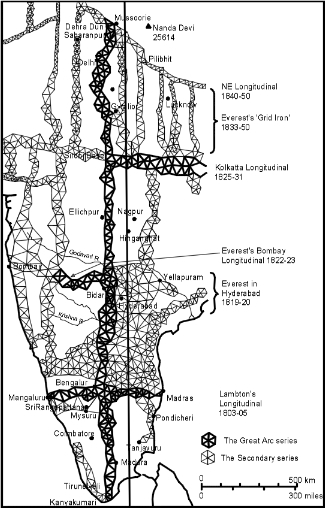
\includegraphics[scale=1.22]{"images/image004.jpg"}
\caption{ಗ್ರೇಟ್ ಆರ್ಕ್ ಸರಣಿ}\label{chap3-fig02}
\end{figure}

ಈ ಟ್ರೈಯಾಂಗ್ಯುಲೇಷನ್​ ಬಿಂದುಗಳನ್ನು ‘ಗ್ರೇಟ್​ ಟ್ರಿಗನಮಿಟ್ರಿಕಲ್​ ಸರ್ವೇ ಸ್ಟೇಷನ್​\break ಗಳು’ ಅಥವಾ ‘ಜಿಟಿಎಸ್​’ಗಳು ಎಂದು ಸಾಮಾನ್ಯವಾಗಿ ಕರೆಯುತ್ತಾರೆಂದು ನಮಗೆ ತಿಳಿದಿದೆ. ಈ ಜಿಟಿಎಸ್​ಗಳು ಇರುವುದೇ ಬೆಟ್ಟದ ಮೇಲಿನ ಅಥವಾ ಪರ್ವತ ಶಿಖರದ ಮೇಲಿನ ನಿರ್ಜನ ಪ್ರದೇಶದಲ್ಲಿ. ಈ ಜಿಟಿಎಸ್​ ಪಾಯಿಂಟ್​ಗಳೇ ಸಾಮಾನ್ಯವಾಗಿ ಜನರು ನೋಡುವ, ಅವರು ಬಳಸುವ, ಟೋಪೋಗ್ರಫಿಕಲ್​ ಸರ್ವೇ ಮತ್ತು ಕೆಡಸ್ಟ್ರಲ್​ ಸರ್ವೇ ಮ್ಯಾಪಿಂಗ್​ ಕಾರ್ಯಗಳಿಗೆ ಆರಂಭ ಬಿಂದುಗಳಾಗಿ, ಆಧಾರ ಬಿಂದುಗಳಾಗಿ, ನಿಯಂತ್ರಣ ಬಿಂದುಗಳಾಗಿ ಕೆಲಸ ನಿರ್ವಹಿಸುತ್ತವೆ. ಟೋಪೋಗ್ರಫಿಕಲ್​ ಸರ್ವೇಗೆ ಹಾಗೂ ಕೆಡಸ್ಟ್ರಲ್​ ಸರ್ವೇಗೆ ಈ ಟ್ರಿಗನಮಿಟ್ರಿಕಲ್​ ಸರ್ವೇ ಸ್ಟೇಷನ್​ಗಳೇ ಬೆನ್ನೆಲುಬು, ಆಧಾರಸ್ತಂಭ. ಈ ಜಿಟಿಎಸ್​ ನಿಲ್ದಾಣಗಳ\break ಸರಣೀ ಪಟ್ಟಿಯ ಹಂದರದ ಮೇಲೆ ಟೋಪೋಗ್ರಫಿಕಲ್​ ಸರ್ವೇಯ ಮತ್ತು ಕೆಡಸ್ಟ್ರಲ್​ ಸರ್ವೇಯ ಭೂ ವಿವರದ ಚಿತ್ರವನ್ನು ಹೊದಿಸಲಾಗುತ್ತದೆ. ಯಾವುದೇ ಮರಕ್ಕೆ ಜಿಟಿಎಸ್​ ಬಿಂದುಗಳು ಬೇರು ಬುಡವಾದರೆ, ಈ ಬೇರು ಬುಡವನ್ನು ಆಶ್ರಯಿಸಿ ಭದ್ರವಾಗಿ, ವಿಶಾಲವಾಗಿ ಬೆಳೆದ ಟೋಪೋಗ್ರಫಿಕಲ್​ ಮತ್ತು ಕೆಡಸ್ಟ್ರಲ್​ ಮ್ಯಾಪುಗಳು ಹೊರ ನೋಟಕ್ಕೆ ನಮ್ಮ ಕಣ್ಣಿಗೆ ಕಾಣುವ ಮರದ ರೆಂಬೆ ಕೊಂಬೆಗಳು ಎನ್ನಬಹುದು.

ಟ್ರಿಗನಮಿಟ್ರಿಕಲ್​ ಸರ್ವೇಯಲ್ಲಿ, ಟ್ರೈಯಾಂಗ್ಯುಲೇಷನ್​ ಕಾರ್ಯವನ್ನು, ಆರಂಭದಲ್ಲಿ, ಗರಿಷ್ಟ ನಿಖರತೆಯಿಂದ ನಿಗದಿ ಮಾಡಲಾಗುತ್ತದೆ. ಈ ಆರಂಭಿಕ ಹಂತದಲ್ಲಿ ಮೂಡಿದ ತ್ರಿಭುಜಗಳು ಪ್ರಾಥಮಿಕ ತ್ರಿಭುಜ ಬಿಂದುಗಳಾಗಿರುತ್ತವೆ. ಆದರೆ ಈ ಆರಂಭಿಕ ಜಿಟಿಎಸ್​ ಬಿಂದುಗಳು, ಗುಡ್ಡದ ಮೇಲೆ, ಬೆಟ್ಟದ ಮೇಲೆ ಒಂದಕ್ಕೊಂದು ಸುಮಾರು \enginline{30–40} ಮೈಲುಗಳ ದೂರದಲ್ಲಿ ಇರುತ್ತವೆ. ಡೀಟೈಲ್​ ಸರ್ವೇಗೆ ಪ್ರಾರಂಭಿಕ ಬಿಂದುಗಳು ಇನ್ನೂ ಹತ್ತಿರ ಹತ್ತಿರದಲ್ಲಿ ಇರಬೇಕಾಗುತ್ತದೆ. \enginline{30–40} ಮೈಲುಗಳಷ್ಟು ಪರಸ್ಪರ ದೂರದಲ್ಲಿ ವಿರಳವಾಗಿರುವ ಬಿಂದುಗಳನ್ನು ಹೆಚ್ಚಿಸಿಕೊಳ್ಳಬೇಕಾಗುತ್ತದೆ. ಸೂಕ್ತ ವಿಧಾನದಲ್ಲಿ ಈ ಪ್ರಾಥಮಿಕ ತ್ರಿಭುಜಗಳನ್ನು ಪುನಹ ಸಣ್ಣ ಸಣ್ಣ ತ್ರಿಭುಜಗಳನ್ನಾಗಿ ವಿಭಜಿಸಿಕೊಳ್ಳಬೇಕು. ಇದನ್ನು ‘ಸೆಕೆಂಡರೀ ಟ್ರೈಯಾಂಗ್ಯುಲೇಶನ್​’ ಎನ್ನುತ್ತಾರೆ. ಮುಂದುವರೆದು ಈ ಸೆಕೆಂಡರಿ ತ್ರಿಭುಜಗಳನ್ನು ಪುನಹ ಸಣ್ಣ ಸಣ್ಣ ತ್ರಿಭುಜಗಳನ್ನಾಗಿ ವಿಭಜಿಸಿಕೊಳ್ಳಬೇಕು. ಇವುಗಳನ್ನು ‘ಟರ್ಸಿಯರೀ ಟ್ರೈಯಾಂಗ್ಯುಲೇಶನ್​’ ಎನ್ನುತ್ತಾರೆ. ಈ ಬಿಂದುಗಳು ಟೋಪೋಗ್ರಫಿಕಲ್​ ಮತ್ತು ಕೆಡಸ್ಟ್ರಲ್​ ಸರ್ವೇಯರುಗಳಿಗೆ ಭೂಪ್ರದೇಶದ ವಿವರಗಳನ್ನು ತುಂಬಲು ಆರಂಭಿಕ ಬಿಂದುಗಳಾಗುತ್ತವೆ. ಹಾಗೂ ಟೋಪೋಗ್ರಫಿಕಲ್​ ಮತ್ತು ಕೆಡಸ್ಟ್ರಲ್​ ಸರ್ವೇ ಕಾರ್ಯದ ನಿಖರತೆಯ ಪರಿಶೀಲನೆಗೂ ಈ ಟ್ರೈಯಾಂಗ್ಯುಲೇಷನ್​ ಬಿಂದುಗಳು ಸಹಾಯ ಮಾಡುತ್ತವೆ. ಜಿಟಿಎಸ್​ ಬಿಂದುಗಳು ಸರ್ವೇಯರುಗಳಿಗೆ ಅಳತೆ ಆರಂಭಿಸಲು ಅಗತ್ಯವಾದ ನಾಲ್ಕು ಪ್ರಮುಖವಾದ ಅಂಶಗಳನ್ನು ನೀಡುತ್ತವೆ. \enginline{1}. ಅಕ್ಷಾಂಶ, ರೇಖಾಂಶ \enginline{2}. ಬೇಸ್‌ಲೈನ್​ \enginline{3}. ನೈಜ ಉತ್ತರ ದಿಕ್ಕು \enginline{4}. ಸರಾಸರಿ ಸಮುದ್ರ ಮಟ್ಟದಿಂದ ಆ ಬಿಂದುವಿನ ಎತ್ತರ.

ಈ ಗ್ರೇಟ್​ ಟ್ರಿಗನಮಿಟ್ರಿಕಲ್​ ಸರ್ವೇಯು ದೇಶದ ಉದ್ದಗಲಕ್ಕೂ ನಿಖರವಾಗಿ ನಿರ್ಧರಿಸಲ್ಪಟ್ಟ ತ್ರಿಭುಜಗಳ ಸರಣಿಯ ಅಡ್ಡ ಉದ್ದ ಸಾಲುಗಳ ಜಾಲವಾಗಿದೆ. ಗ್ರೇಟ್​ ಆರ್ಕ್‌ನ ಒಂದಕ್ಕೊಂದು ಅಂಟಿದ ತ್ರಿಭುಜಗಳ ಜಾಲದ ಪಟ್ಟಿಯು, ದಕ್ಷಿಣದ ಕನ್ಯಾಕುಮಾರಿಯಿಂದ ಉತ್ತರದ ಮಸೂರಿಯವರೆಗೆ ವ್ಯಾಪಿಸಿದೆ. ಈ ಮುಖ್ಯ ಗ್ರೇಟ್​ ಆರ್ಕ್ ಜಾಲವನ್ನು ಪ್ರಾಥಮಿಕ ಸರಣಿ ಎನ್ನುವರು. ನಂತರದ ಪೂರ್ವ–ಪಶ್ಚಿಮ ಮತ್ತು ಉತ್ತರ–ದಕ್ಷಿಣ ಸಹಾಯಕ ಜಾಲಗಳಿಗೆ ಈ ಪ್ರಧಾನ ಗ್ರೇಟ್​ ಆರ್ಕ್ ಜಾಲವು ಮುಖ್ಯ ಆಧಾರವನ್ನು ಒದಗಿಸಿದೆ. ಚಿತ್ರದಲ್ಲಿ ಟ್ರೈಯಾಂಗ್ಯುಲೇಷನ್​ ಜಾಲವನ್ನು ಗಮನಿಸಬಹುದು.

